% Define document class
%\documentclass[twocolumn]{aastex631}
\documentclass[modern]{aastex631}

% Some entries inspired from a preamble by Adrian Price-Whelan, https://github.com/adrn/PhaseSpiralAsteroseismology/blob/main/tex/preamble.tex

\usepackage{showyourwork}

% Latex imports
\let\tablenum\relax             % necessary for AASTeX
\usepackage{siunitx}
\sisetup{range-phrase=-, range-units=single, separate-uncertainty=true}
\sisetup{separate-uncertainty=true}
\usepackage{blindtext}          % Filler text
\usepackage{xcolor}

% paper comments
\usepackage{comment}						 % comments that can be switched visible/invisible
\includecomment{comment}
%\specialcomment{outtake}{\begingroup\sffamily\color{gray}}{\endgroup}
\specialcomment{note}{\begingroup\sffamily\color{red!40!green!70!blue!90}}{\endgroup}
%\excludecomment{note}                       % switch notes off

%% switch TODO notes on/off
\usepackage[backgroundcolor=red!20!green!40!blue!10, textsize=tiny]{todonotes}
\usepackage{regexpatch}
\makeatletter
\xpatchcmd{\@todo}{\setkeys{todonotes}{#1}}{\setkeys{todonotes}{inline,#1}}{}{}
\makeatother
%\usepackage[disable]{todonotes}			% switches all todo notes to invisible

% ---------------------------------
% PAPER VARIABLES
\newcommand{\Nplanets}{\ensuremath{733}}
\newcommand{\percentageTransiting}{999}
\newcommand{\dmax}{\ensuremath{50\,\mathrm{pc}}}
\newcommand{\wrr}{0.001}
\newcommand{\windowsize}{25}
\newcommand{\prSmin}{10}
\newcommand{\prSmax}{1000}
\newcommand{\prWRRmin}{10^{-5}}
\newcommand{\prWRRmax}{0.1}
\newcommand{\prRmin}{0.1}
\newcommand{\prRmax}{15}


% ---------------------------------
% CONSTANTS/MISSIONS/ABBREVIATIONS

% SIunitx definitions
\DeclareSIUnit\mSun{M_\odot}
\DeclareSIUnit\Msun{M_\odot}
\DeclareSIUnit\mStar{M_\star}
\DeclareSIUnit\Mstar{M_\star}
\DeclareSIUnit\mEarth{M_\oplus}
\DeclareSIUnit\Mearth{M_\oplus}
\DeclareSIUnit\rEarth{R_\oplus}
\DeclareSIUnit\Rearth{R_\oplus}
\DeclareSIUnit\year{yr}
\DeclareSIUnit\au{au}
\DeclareSIUnit\dex{dex}
\DeclareSIUnit\ppm{ppm}
\DeclareSIUnit\eV{eV}

% Missions/Projects/Packages
\newcommand{\project}[1]{\textsl{#1}}
\newcommand{\rst}{\project{Nancy Grace Roman Space Telescope}}
\newcommand{\plato}{\project{PLATO}}
\newcommand{\cheops}{\project{CHEOPS}}
\newcommand{\kepler}{\project{Kepler}}
\newcommand{\emcee}{\project{emcee}}

% Stats / probability
\newcommand{\given}{\,|\,}
\newcommand{\norm}{\mathcal{N}}
\newcommand{\pdf}{\textsl{pdf}}

% Maths
\newcommand{\dd}{\mathrm{d}}
\newcommand{\transpose}[1]{{#1}^{\mathsf{T}}}
\newcommand{\inverse}[1]{{#1}^{-1}}
\newcommand{\argmin}{\operatornamewithlimits{argmin}}
\newcommand{\mean}[1]{\left< #1 \right>}

% Non-scalar variables
\renewcommand{\vec}[1]{\ensuremath{\bs{#1}}}
\newcommand{\mat}[1]{\ensuremath{\mathbf{#1}}}

% Unit shortcuts
\newcommand{\msun}{\ensuremath{\mathrm{M}_\odot}}
\newcommand{\mjup}{\ensuremath{\mathrm{M}_{\mathrm{J}}}}
\newcommand{\kms}{\ensuremath{\mathrm{km}~\mathrm{s}^{-1}}}
\newcommand{\mps}{\ensuremath{\mathrm{m}~\mathrm{s}^{-1}}}
\newcommand{\pc}{\ensuremath{\mathrm{pc}}}
\newcommand{\kpc}{\ensuremath{\mathrm{kpc}}}
\newcommand{\kmskpc}{\ensuremath{\mathrm{km}~\mathrm{s}^{-1}~\mathrm{kpc}^{-1}}}
\newcommand{\dayd}{\ensuremath{\mathrm{d}}}
\newcommand{\yr}{\ensuremath{\mathrm{yr}}}
\newcommand{\AU}{\ensuremath{\mathrm{AU}}}
\newcommand{\Kel}{\ensuremath{\mathrm{K}}}

% Misc.
\newcommand{\bs}[1]{\boldsymbol{#1}}

% Astronomy
\newcommand{\feh}{\ensuremath{{[{\rm Fe}/{\rm H}]}}}
\newcommand{\mh}{\ensuremath{{[{\rm M}/{\rm H}]}}}
\newcommand{\logg}{\ensuremath{\log g}}
\newcommand{\Teff}{\ensuremath{T_{\textrm{eff}}}}
\newcommand{\vsini}{\ensuremath{v\,\sin i}}
\newcommand{\gaia}{\textsl{Gaia}}

% Begin!
\begin{document}

% Title
\title{The imprint of global magma oceans on exoplanet demographics}

% Author list
\author[0000-0001-8355-2107]{Martin Schlecker}
\affiliation{Department of Astronomy/Steward Observatory, The University of Arizona, 933 North Cherry Avenue, Tucson, AZ 85721, USA}
\author{al.}


% Abstract
\begin{abstract}
    $\ldots$ magma oceans $\ldots$

    Here, we assess the ability of space and ground-based telescopes to test this hypothesis using Bioverse, a simulation framework that leverages contextual information from the overall planet population.
    We argue that in the near future, ESA's PLATO mission and NASA's Roman Space Telescope will be the most promising endeavors to constrain this demographic feature.
    For each of these missions, we identify the key mission design drivers that enable a statistically sound detection.
    We also show the unique synergy of these missions in answering this question, and what survey strategy optimizes the statistical power of the combined dataset.

    $\ldots$ its measurement will also provide insights into which stars harbor the nearest habitable worlds.
\end{abstract}

% Main body
\section{Introduction}
Several patterns in the planetary parameter space have been reported in demographic studies or predicted from planet formation theories.
\begin{note}
    ...long-term goal/overarching objective: derive the geophysical history of rocky extrasolar planets.
   ...
\todo[inline]{introduce magma oceans and their influence on planetary radii~\citep{Dorn2021}.}
    ...current/future observations of planets that are currently in the runaway greenhouse phase may constrain properties of their planetary mantles... make connection between interior and atmospheres.
\end{note}

\begin{figure*}
    \begin{centering}
        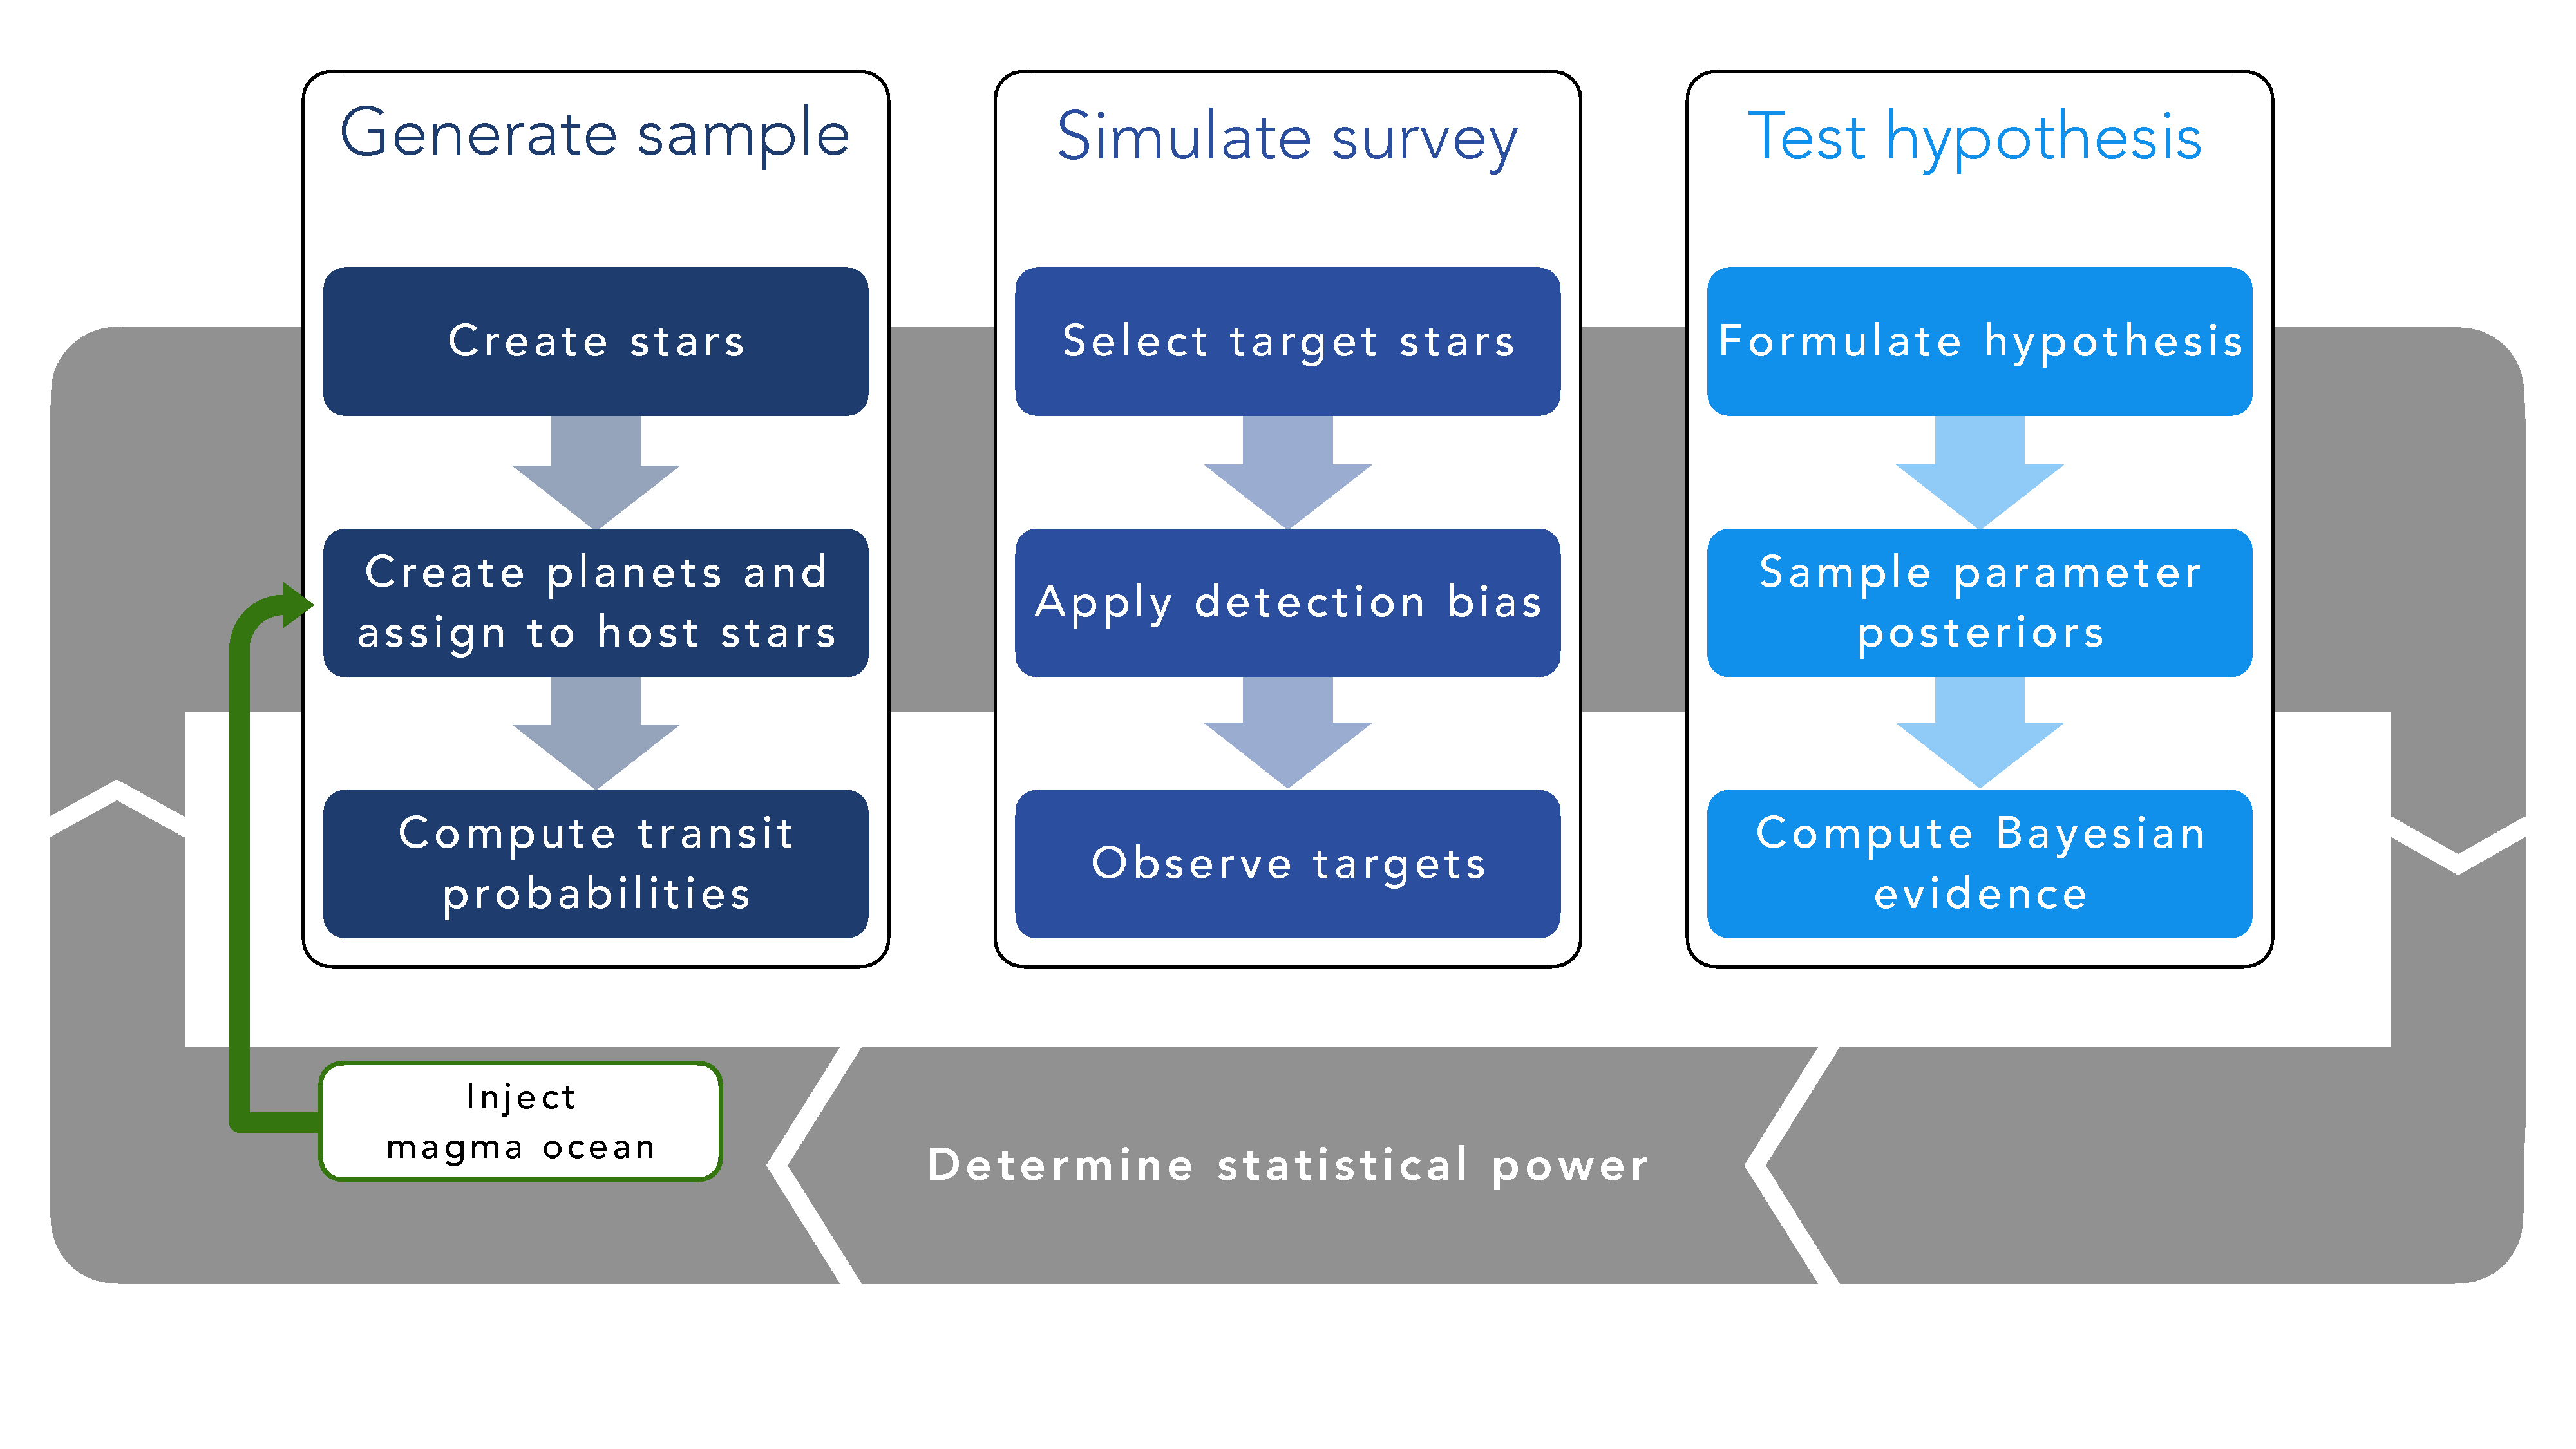
\includegraphics[width=\hsize]{figures/flowchart.pdf}
        \caption{Workflow of our hypothesis testing with Bioverse. In the first block, a stellar sample is generated based on XXX. The stars are then populated with planets from XXX, which may be assigned a magma ocean based on the model described in Sect.~\ref{sec:mo_model}. The planets' respective transit probabilities are computed. The second block simulates the exoplanet survey whereby selection effects and detection biases are introduced. Finally, the third block deals with testing a hypothesis based on the data from the simulated survey. By iterating through these steps, we compute the statistical power of testing the hypothesis given the assumed survey design.}
        \label{fig:flowchart}
    \end{centering}
\end{figure*}


\section{Global magma oceans and their imprint on exoplanet demographics}
\todo[inline]{"Methods Section" for the geophysical models.}
\subsection{Global magma oceans}
\todo[inline]{introduce geophysical model.\\ Introduce its parametrization either here or further down when modeling demographic imprint.\\ Figure~\ref{fig:magmaocean_model} goes here.}

%\begin{figure}
\begin{figure}[!ht]
    \begin{centering}
        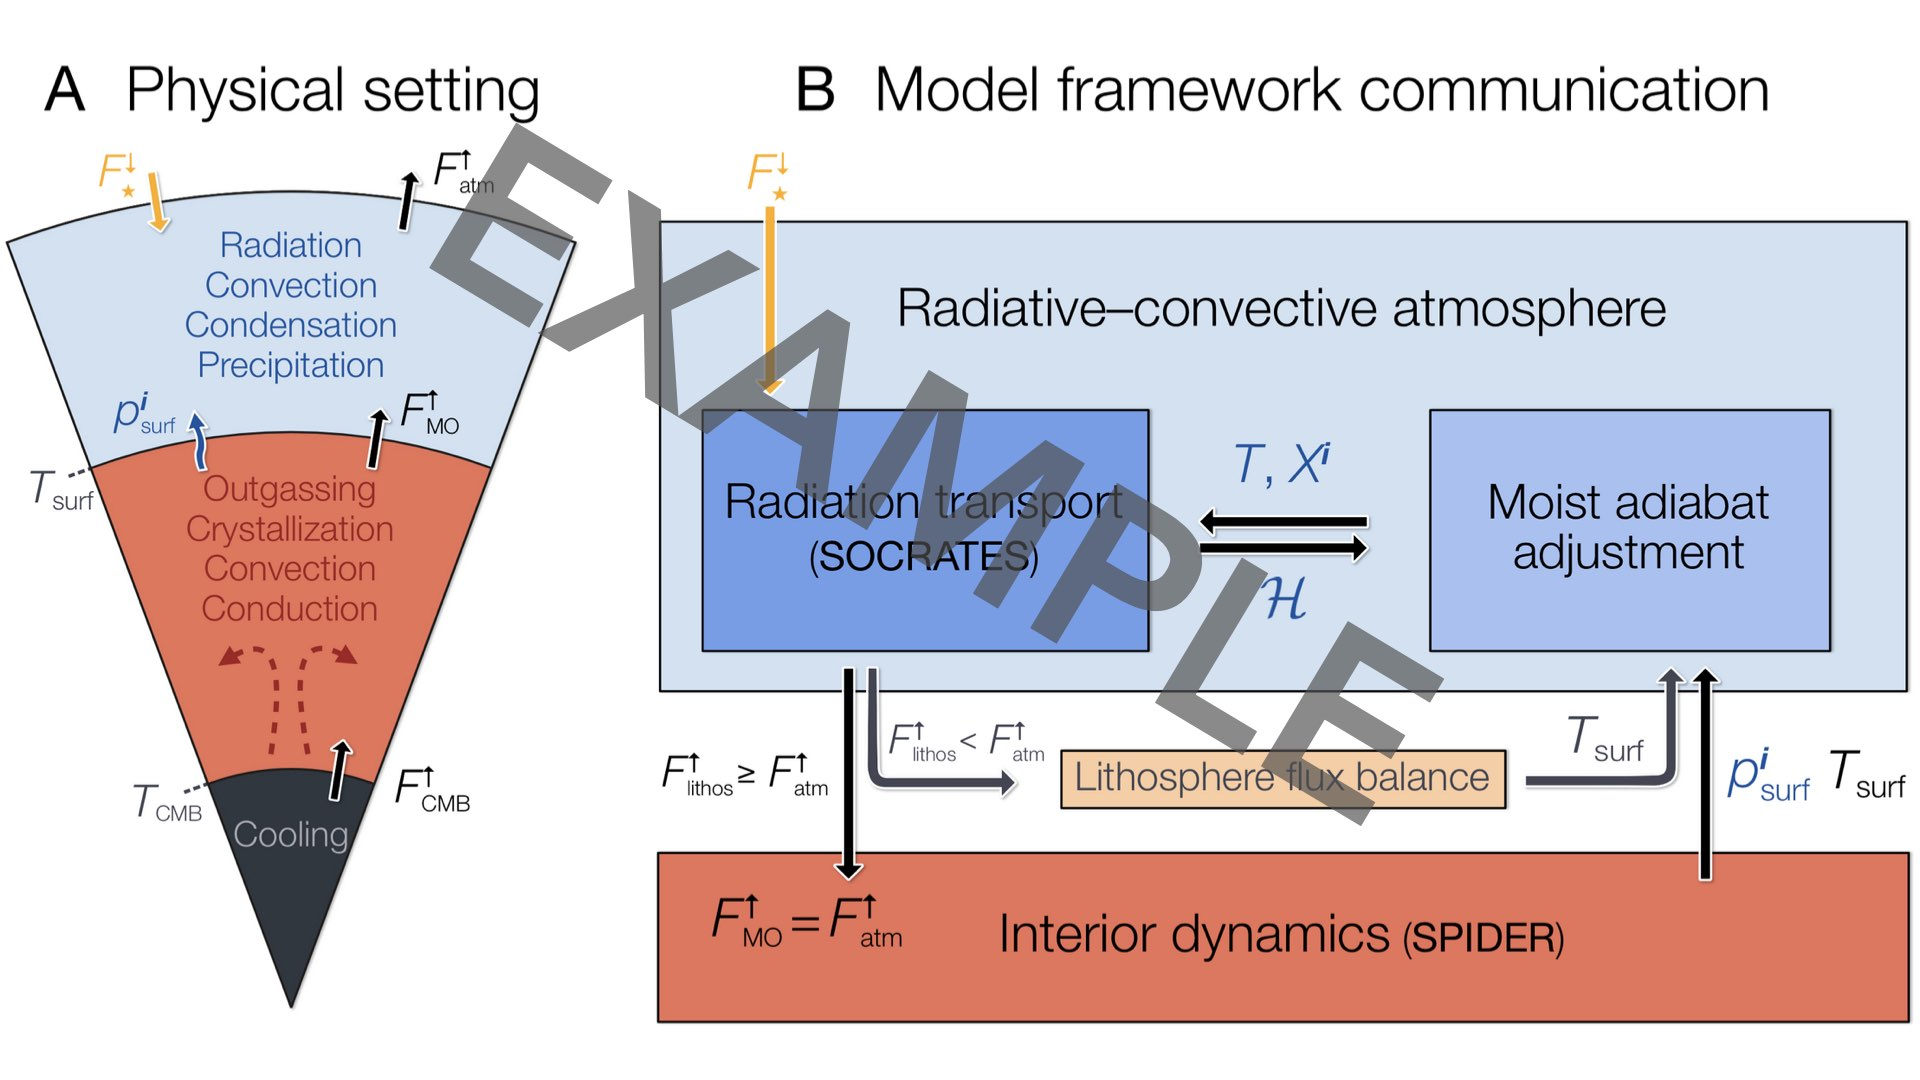
\includegraphics[width=\hsize]{figures/magmaocean_model.jpg}
        \caption{Schematics of the geophysical model framework.}
        \label{fig:magmaocean_model}
    \end{centering}
\end{figure}


\subsection{Demographic imprint of magma oceans}
\todo{describe the expected imprint on the exoplanet population. \\Provide parametrizations from \citet{Dorn2021}'s models.}

\subsubsection{Parametrization}
\label{sec:mo_model}
\todo{specific parametrization, dependency on bulk planet/orbit params (doesn't have to be its own subsubsection)}

\Blindtext[1]


\begin{note}
    The power from the host star per unit area at the position of a planet or stellar insolation $S$ in units of Earth's insolation is given by
    \begin{equation}
        \frac{S}{S_\oplus} = \left(\frac{L_\star}{L_\odot}\right) \left(\frac{au}{a}\right)^2 .
    \end{equation}

    We further define the solar-equivalent semi-major axis $a_{eff} = a (L_\star/L_\odot)^{-1/2}$, at which a planet experiences the same insolation as a Solar System planet at an orbital distance~$a$.
\end{note}





\section{Testing the magma ocean hypothesis}
\todo[inline]{"Methods Section" of the hypothesis testing part. Introduce the idea of constraining magma ocean frequencies and/or physics with Bayesian stats on exoplanet population; introduce Bioverse; report methods of the hypothesis tests.}

\subsection{Synthetic star and planet sample}
\begin{note}
    The first step in our analysis is to generate a synthetic sample of stars and planets.
    First, we create a stellar population based on the observed population in the solar neighborhood, to which we then assign planetary systems based on occurrence rates derived from the \kepler mission.
    In our fiducial model setup, we consider stars with a maximum distance to the solar system of \dmax.
\end{note}

\subsubsection{Stellar sample from Gaia DR3}
\todo{Which star sample was actually used?}

\subsubsection{Planetary ocurrence rates in orbital period and radius}
\todo[inline]{What is the source of our occurrence rate density from which we draw? We could also use a generative model that directly approximates an observed or theoretical density \citep[e.g.,][]{Schlecker2021b}.}
\begin{note}
    The NASA Exoplanet Program Analysis Group chartered Science Analysis Group 13 (SAG 13)...
    The inferred occurrence rate density can be expressed as a power law in planet radius and period
    \begin{equation}
        \frac{\partial^2n}{\partial \log R \, \partial \log P} = \Gamma R^{\alpha} P^{\beta}
    \end{equation}
that is broken in planet radius, resulting in the free parameters $\Gamma$, $\alpha$, $\beta$, and a breakpoint radius $R_\mathrm{break}$.
\end{note}

\subsubsection{Transit probability}
\todo[inline]{describe how we model inclinations and transits of synthetic planets}
\begin{note}
    Not all planets are transiting from our point of view.
    We model the occurrence of transits by assuming random, isotropic orientations of planetary orbits and calculating the transit impact parameter $b = \cos(i)/R_\star$ for each planet.
    Only planets with $|b| < 1$ are transiting and further considered.
    For these cases we calculate the transit depth
    \begin{equation}\label{eq:transitdepth}
        \delta = \left( \frac{R_\mathrm{P}}{R_\star} \right)^2
    \end{equation}\todo[inline]{check if transit depth or duration are actually used further down}
    and transit duration
    \begin{equation}\label{eq:transitduration}
        t_{\mathrm{T}} = \frac{R_\star P}{\pi a} \sqrt{1 - b^2},
    \end{equation}
    which are relevant for the detection probability of the respective planet~(see Sect.~\ref{sec:sensitivity}).
    After excluding all non-transiting planets, the size of our nominal sample of potentially observable planets drops to $N = \Nplanets$.
\end{note}




\subsubsection{Synthetic planet populations with and without magma oceans}
\todo{describe the way we inject magma oceans into the synthetic planet population with Bioverse}
\begin{figure*}
    \begin{centering}
        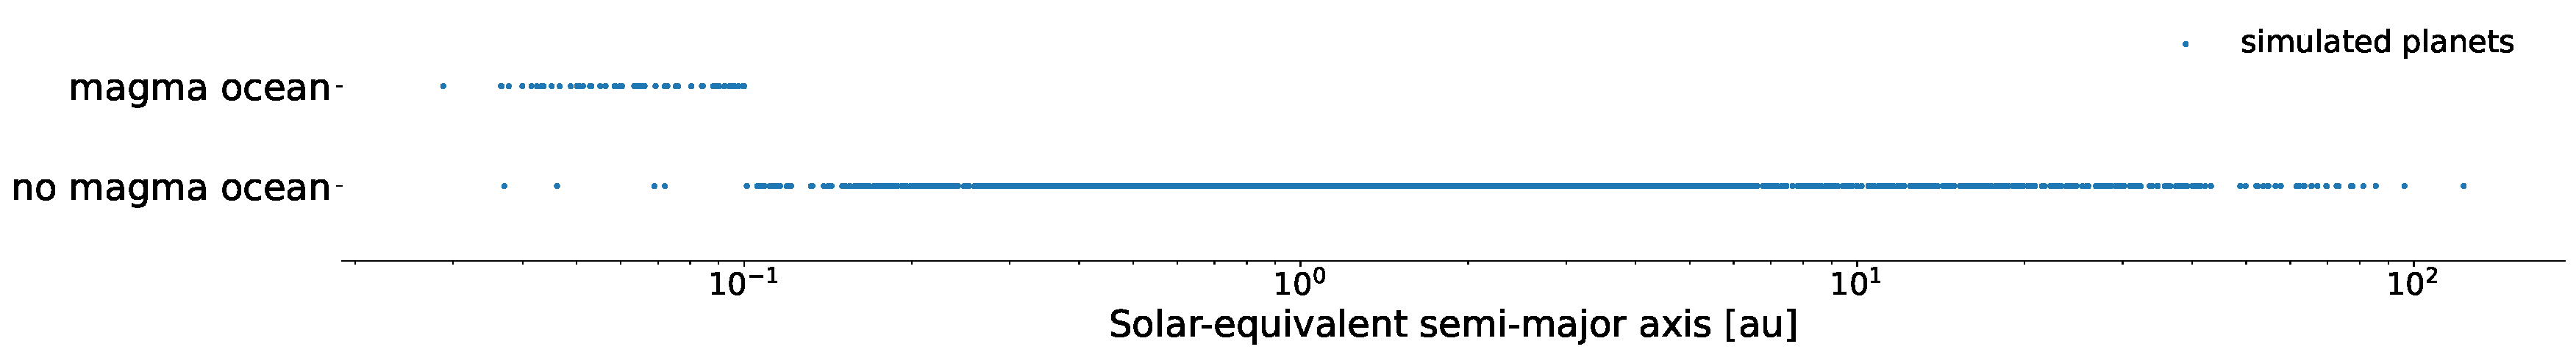
\includegraphics[width=\hsize]{figures/has_magmaocean.pdf}
        \caption{Synthetic planets with and without magmaoceans as a function of Solar-equivalent semi-major axis}
        \label{fig:has_magmaocean}
    \end{centering}
\end{figure*}



\begin{note}
\todo[inline]{Transition to tests of the trend:}
Figure~\ref{fig:has_magmaocean} shows that the subpopulation of planets with magma oceans is apparent in the synthetic dataset.
    In the following, we test if and under what conditions this effect is large enough to be detected with high significance.
\end{note}

\subsection{Testing the magma ocean hypothesis with current and planned exoplanet missions}
\todo{Introduce survey simulation(s). PLATO, Ariel, LIFE?, Nautilus\\ What are threshold missions that are able to detect this signal? =>X meter working for Y years, or X' meter working for Y' years => conclusion could be that there is interesting science to do with intermediate size telescope.}

\subsubsection{Definition of the magma ocean hypothesis and null hypothesis}
\todo{Define the null and alternative hypotheses}
...

For the likelihood function, we assumed that the planet radii $R_{\mathrm{P}, i}$ are measured with a normally distributed uncertainty $\sigma_{R_\mathrm{P}, i}$ and adopted a normal distribution
\begin{equation}
    \mathcal{L}(R_\mathrm{P} \mid \boldsymbol{\theta})=\prod_{i}^{N} \frac{1}{\sqrt{2 \pi \sigma_{R_\mathrm{P}, i}^{2}}} \exp \left(-\frac{\left(R_{\mathrm{P}, i}-h\left(\boldsymbol{\theta}, a_{\mathrm{eff}, i}\right)\right)^{2}}{2 \sigma_{R_\mathrm{P}, i}^{2}}\right).
\end{equation}
Here, $h\left(\boldsymbol{\theta}, a_{\mathrm{eff}, i}\right)$ corresponds to the functional form of the magma ocean hypothesis\todo{link to eqn defining the hypothesis} .
We tested this hypothesis against the null hypothesis $h_\mathrm{null} (\theta, R_\mathrm{P}) = \theta$, which states that there is no relationship between the measured planet radii and (scaled) semi-major axes.

\subsection{Signature and testability of the magma ocean hypothesis with a $<nominal telescope size>$ class space telescope survey}

\begin{figure}[ht!]
%    \script{figurescript.py}
    \begin{centering}
        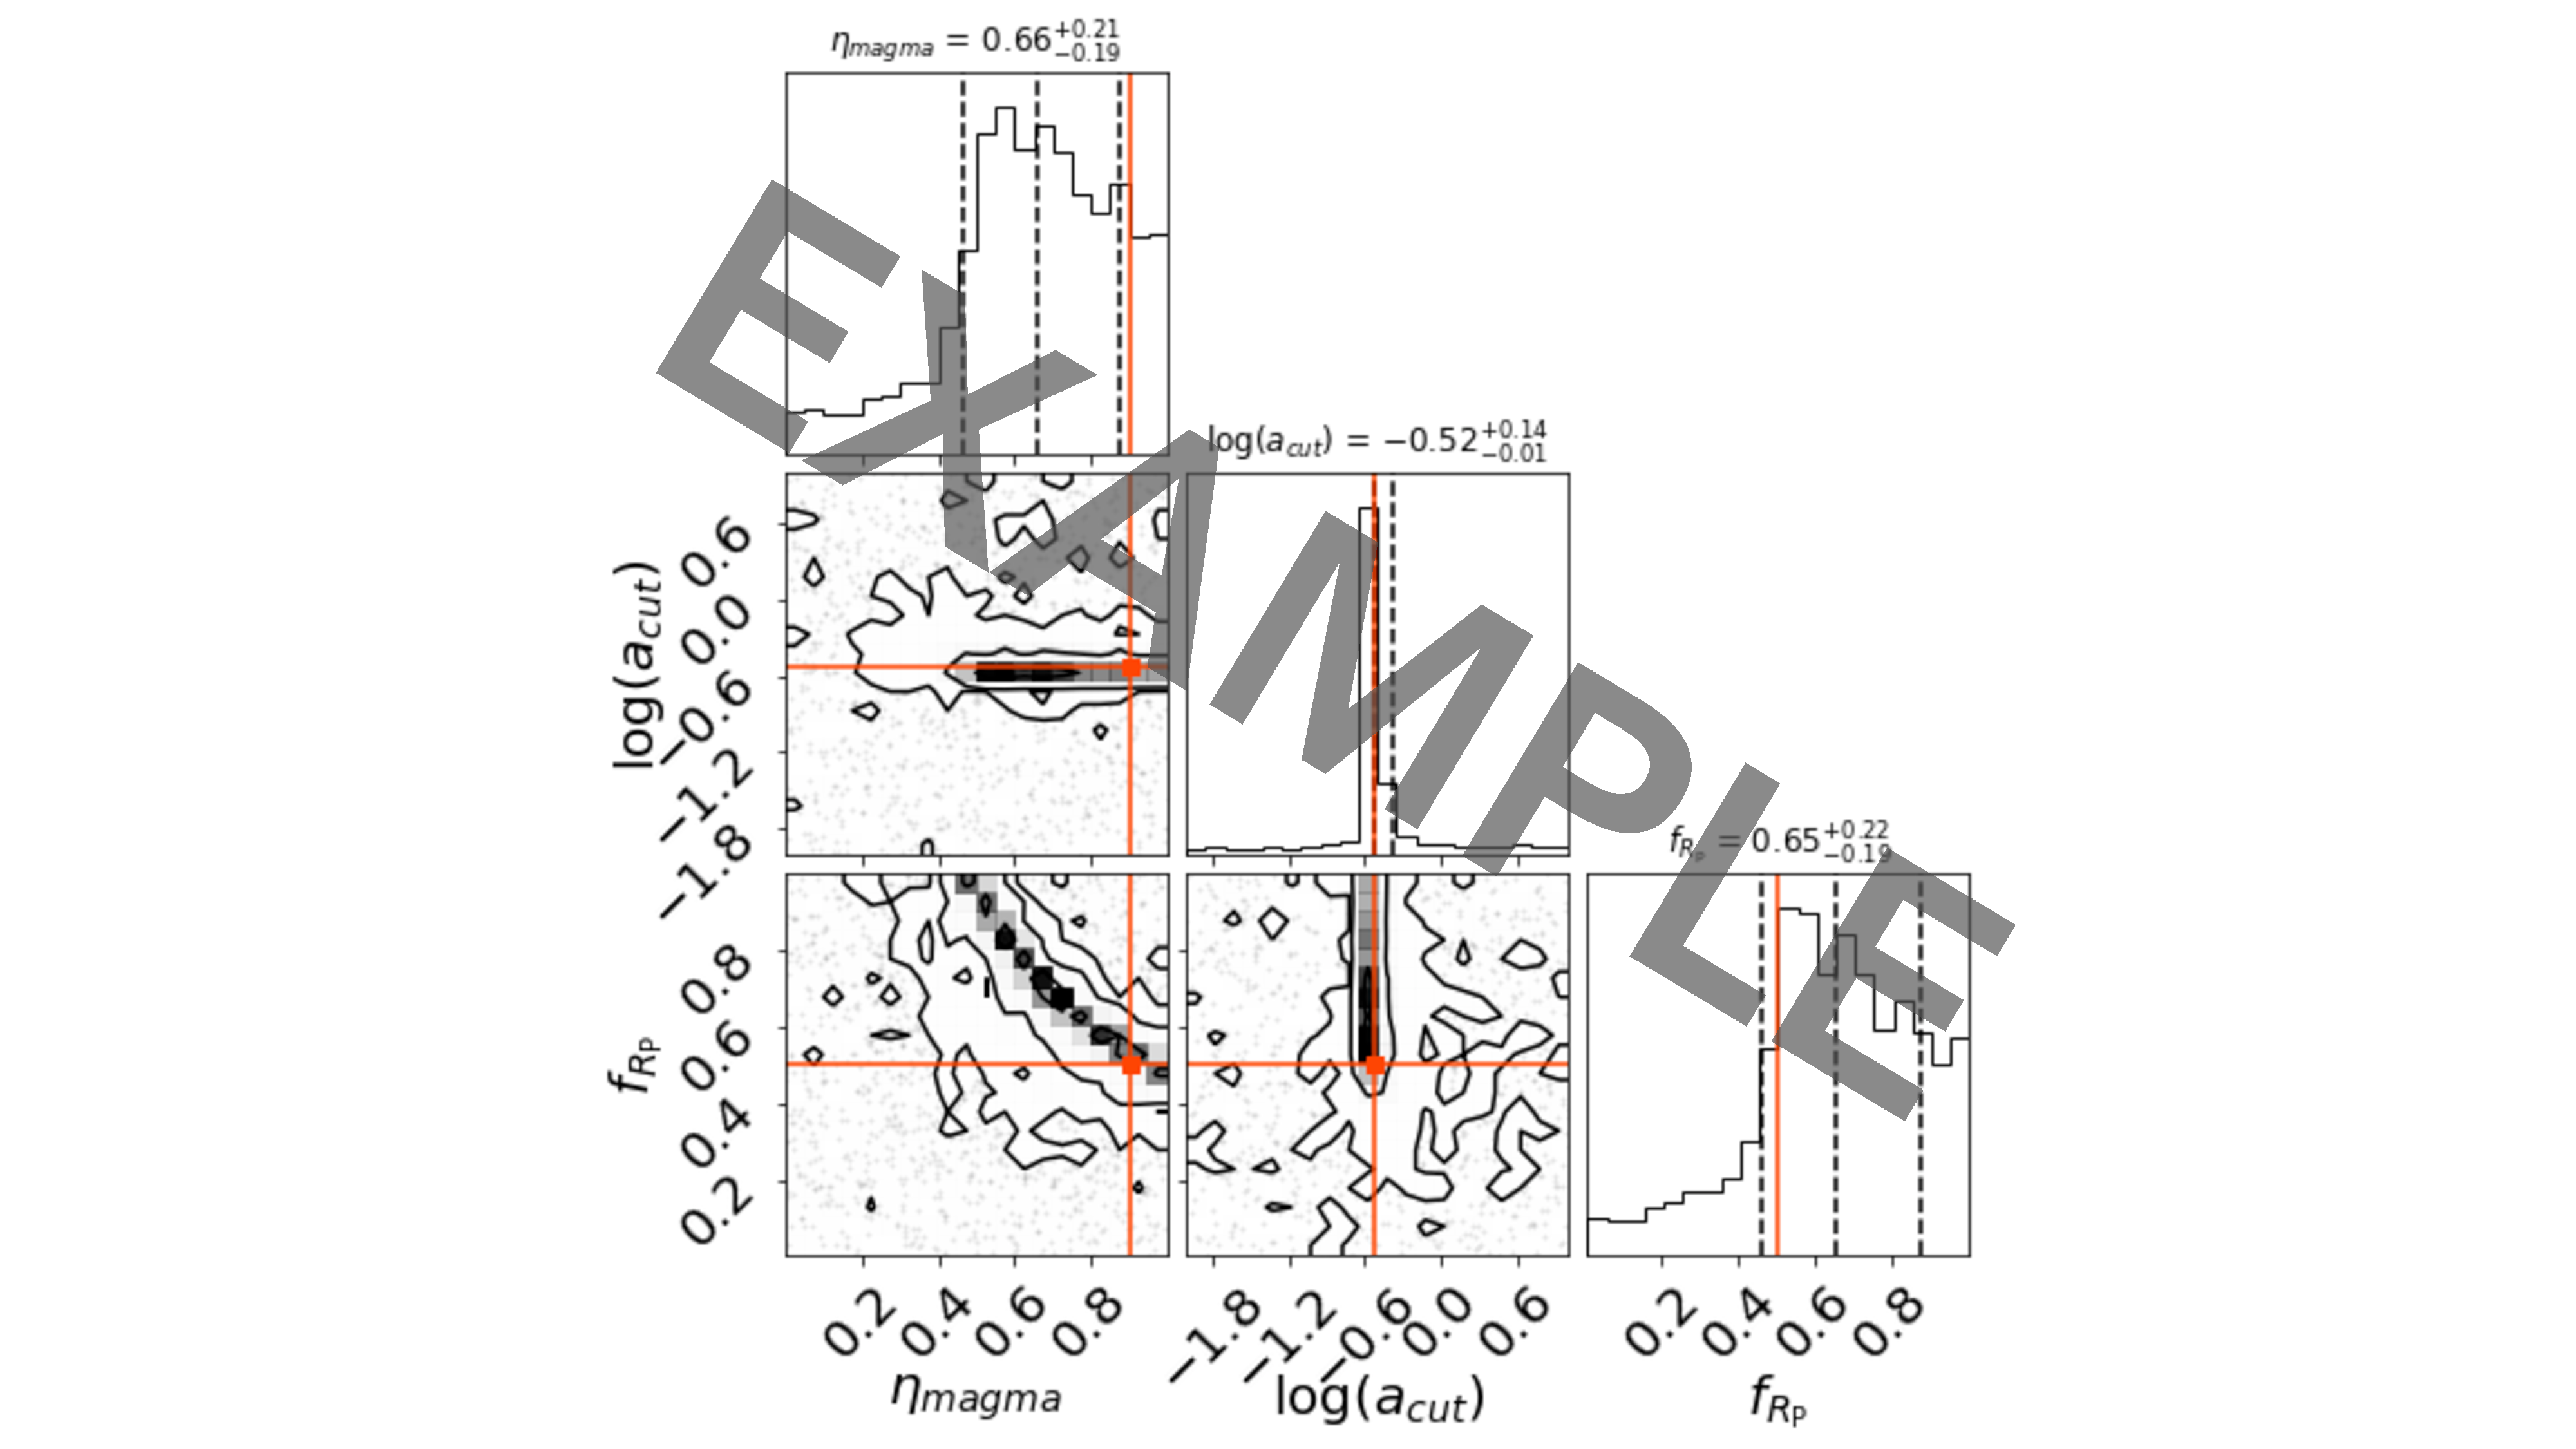
\includegraphics[width=\linewidth]{figures/example_cornerplot.pdf}
        \caption{
        Retrieved posterior distribution of magma ocean model. The density maps in each panel show relationships between and marginalized distributions of the model parameters as they would be retrieved with a targeted $<nominal telescope size>$ survey of $<survey duration>$ duration. True values of the injected magma ocean parameters are shown in orange. ...
        }
        \label{fig:cornerplot}
    \end{centering}
\end{figure}



\begin{note}
   The fidelity of a future detection or falsification of a magma ocean signature will depend on the significance with which the null hypothesis can be excluded.
   As a consequence, instrumentation and survey strategy aiming at testing the hypothesis should aim at maximizing the probability of a true positive detection given the existence of the effect.
   This is called the statistical power of the test.
   Before turning to mission design trades that influence the statistical power in Sect.~\ref{sec:mission-design-trades}, we explore its behavior as a function of various free parameters of the magma ocean model.
    ...
\begin{figure*}[ht!]
%    \script{figurescript.py}
    \begin{centering}
        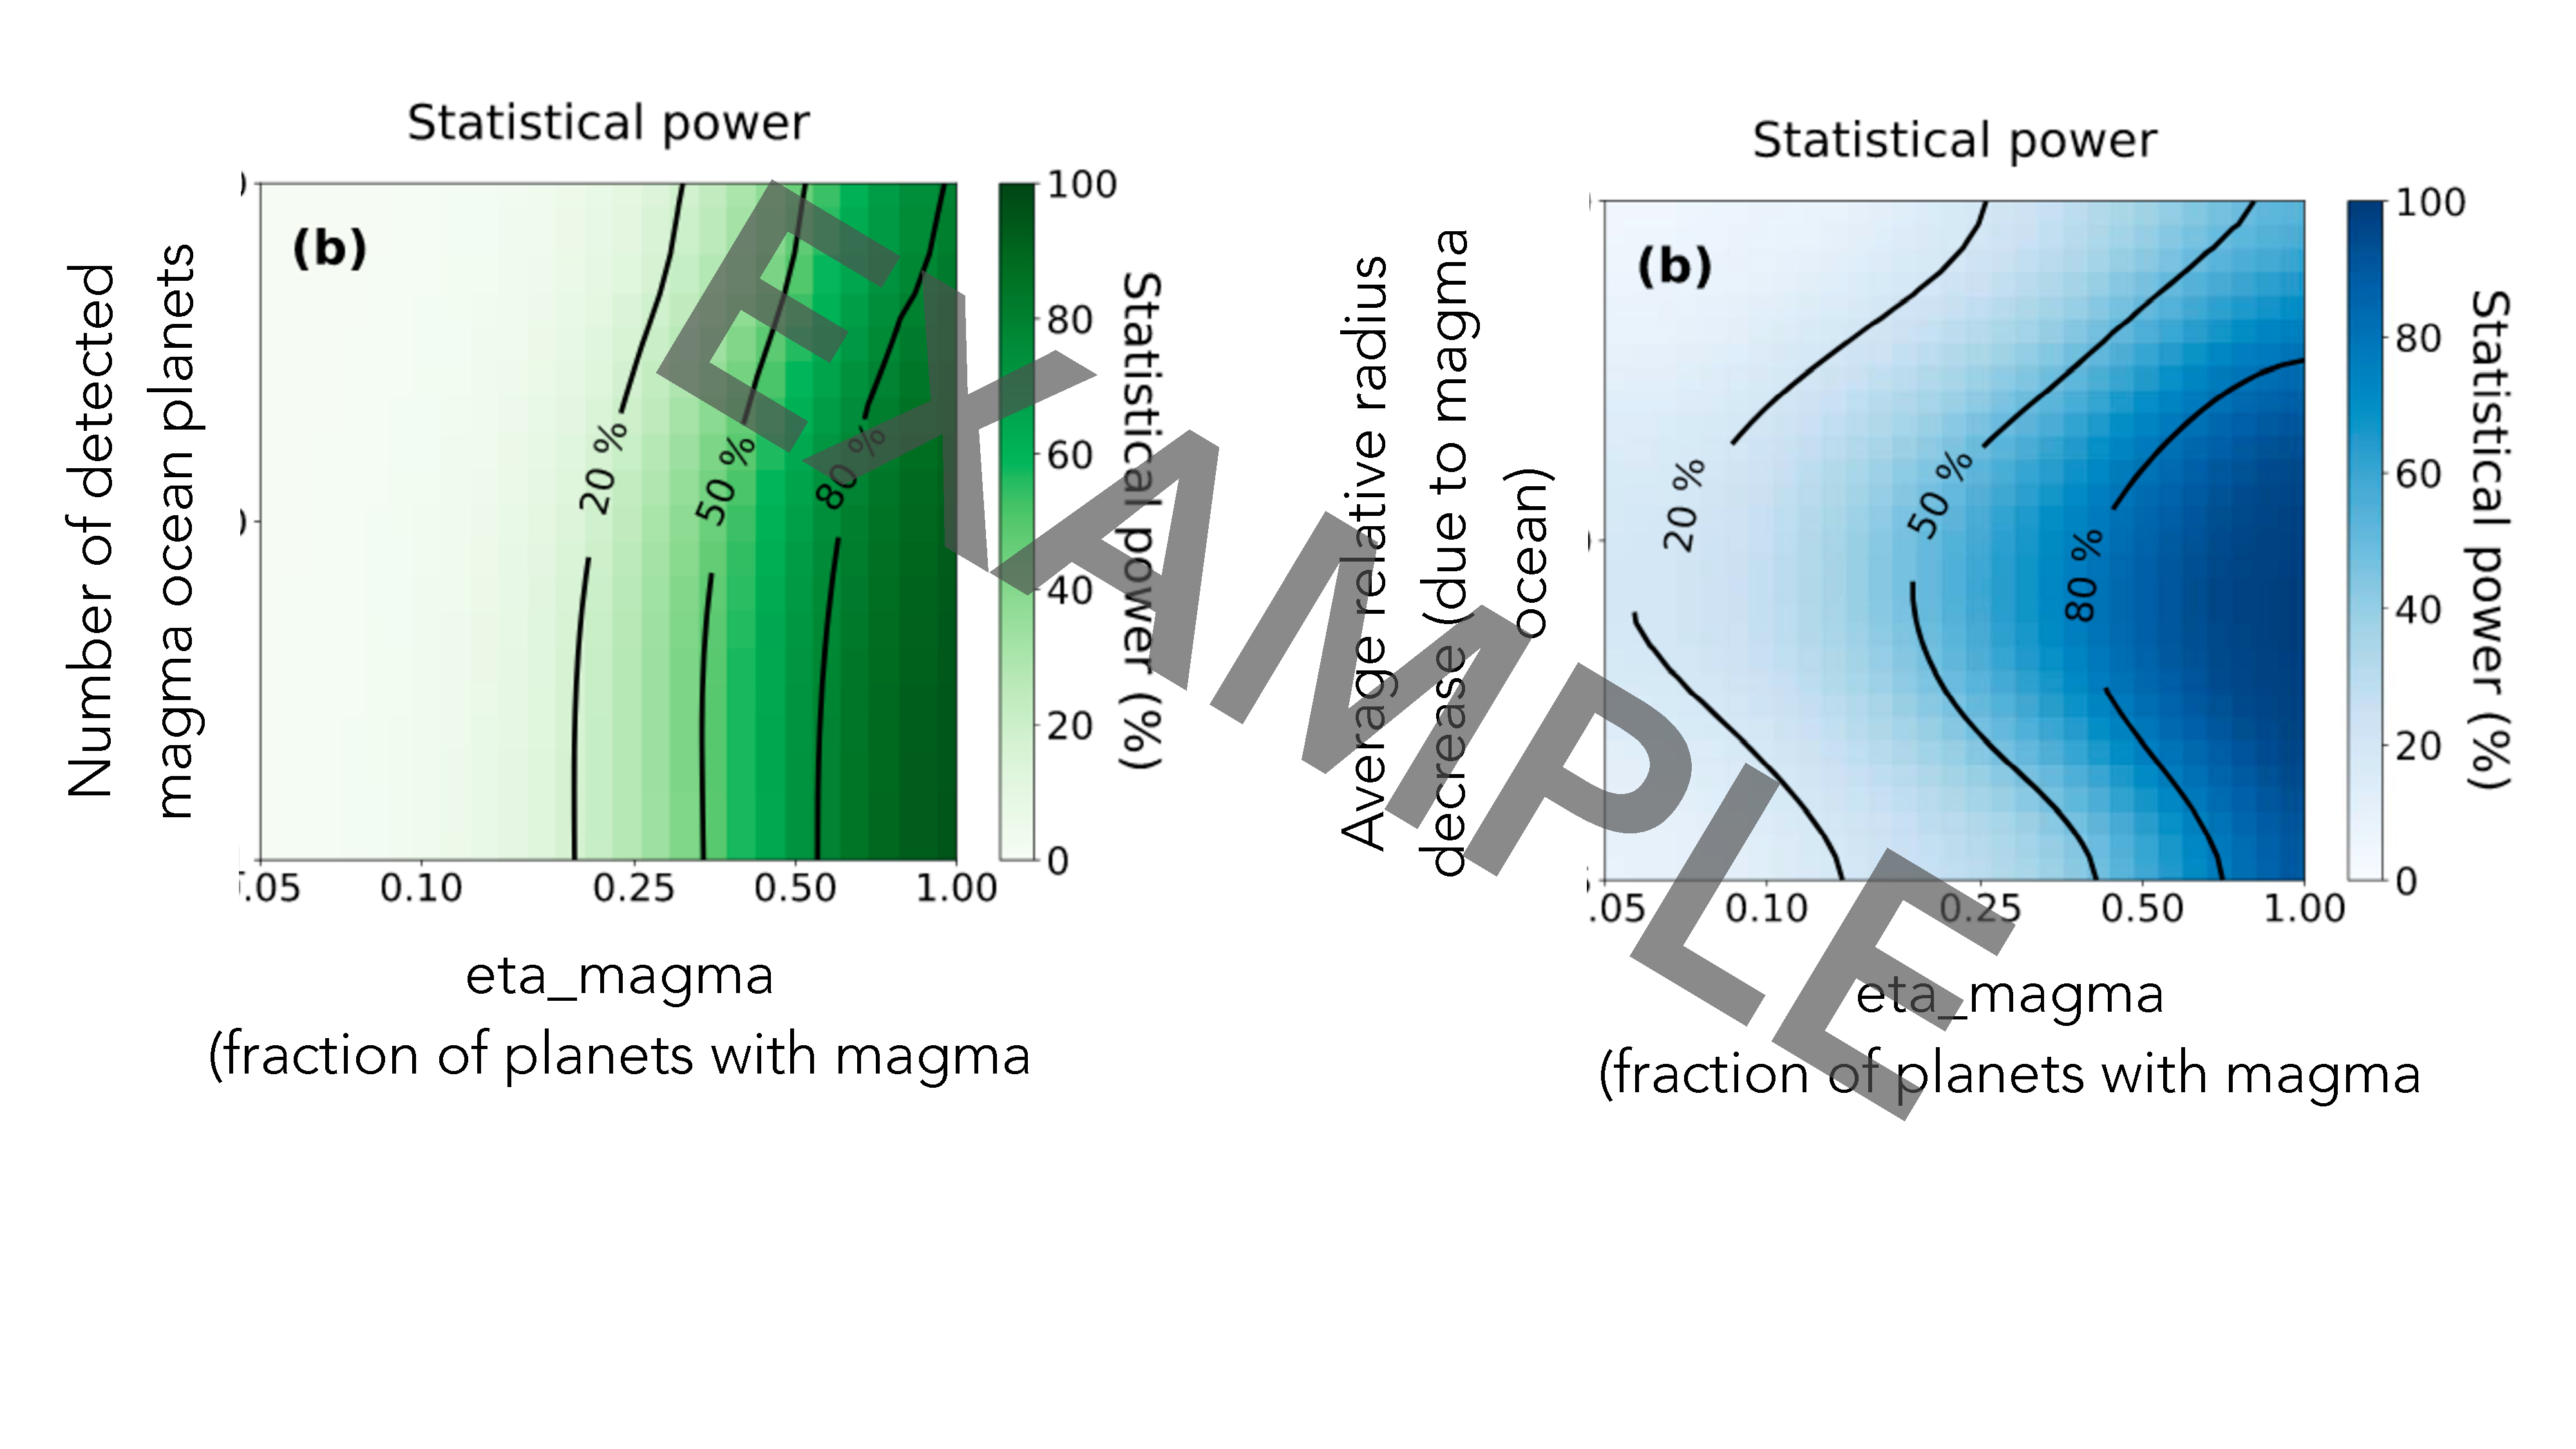
\includegraphics[width=\linewidth]{figures/example_statistical_power.pdf}
        \caption{
        Statistical power of a magma ocean hypothesis test as a function of model parameters.
        }
        \label{fig:statistical_power}
    \end{centering}
\end{figure*}

\end{note}

\subsection{Statistical power of different mission designs}\label{sec:statpower_missions}
\todo[inline]{show detectability of the magma ocean signature for different mission designs}

\begin{figure}[ht!]
%    \script{figurescript.py}
    \begin{centering}

        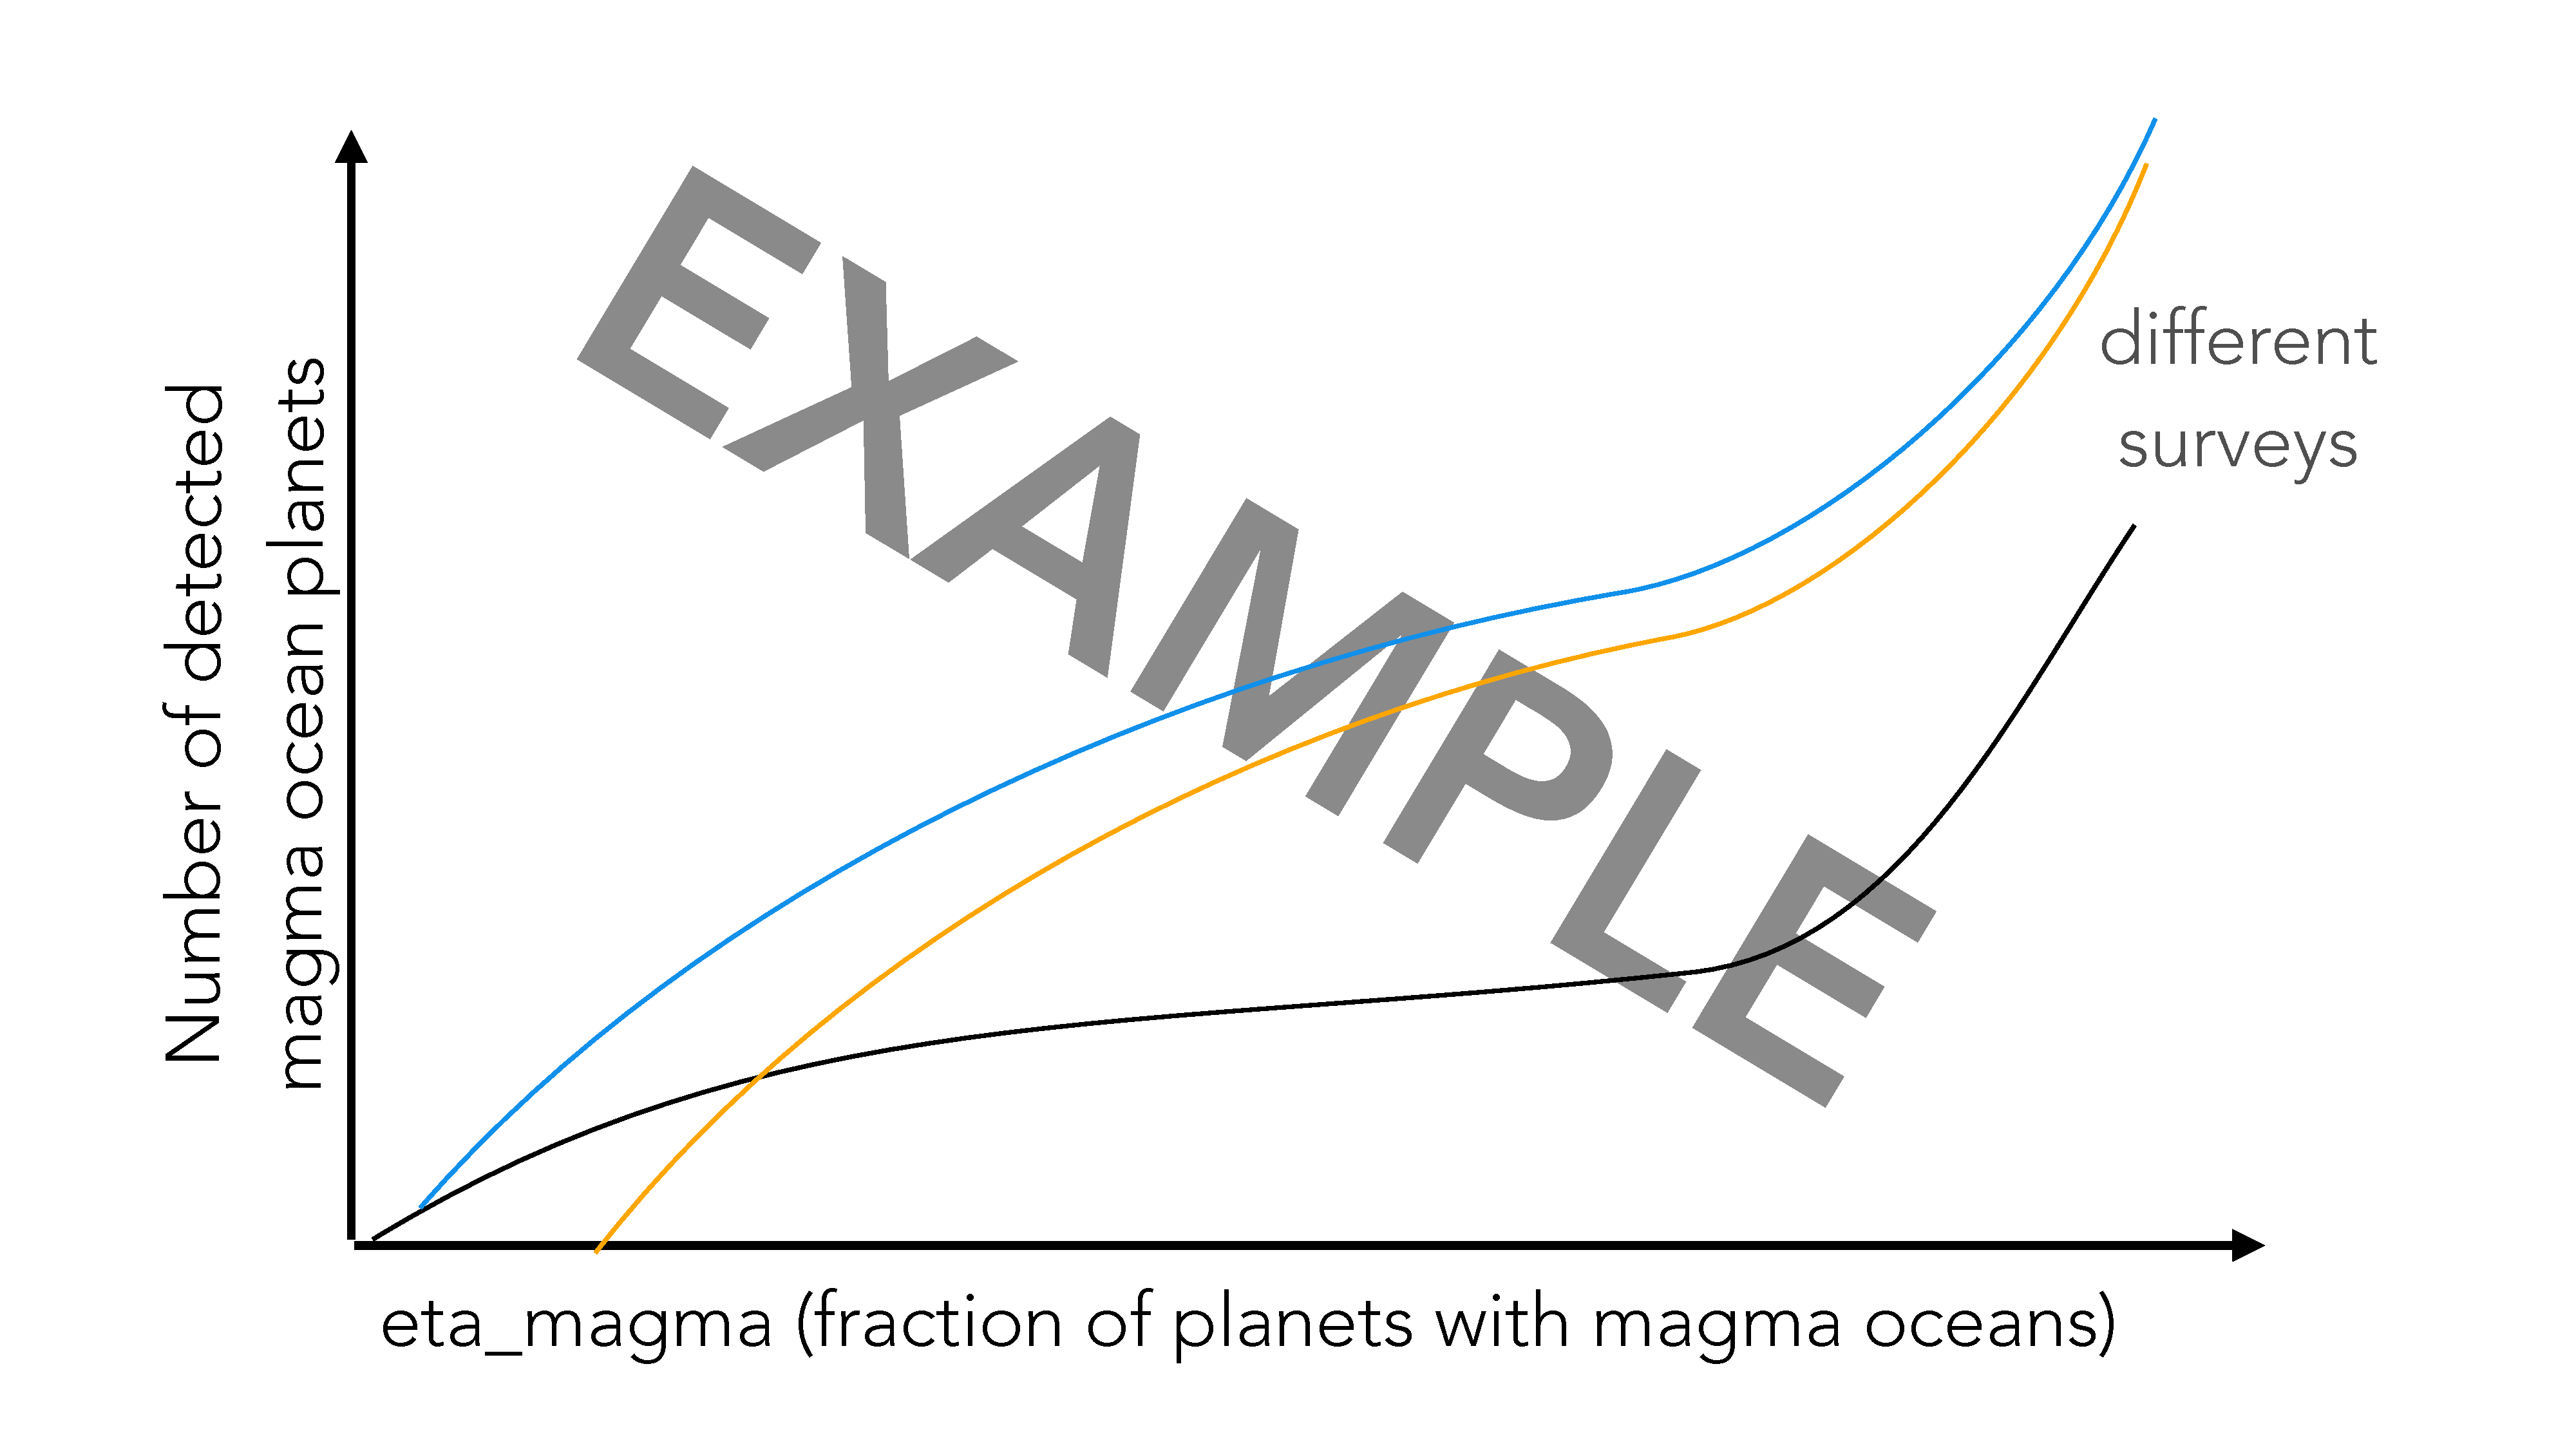
\includegraphics[width=\linewidth]{figures/example_Ndetected_surveys.pdf}
        \caption{
        Detections of magma ocean-bearing planets as a function of magma ocean occurrence for different survey designs.
        }
        \label{fig:example_Ndetected_surveys}
    \end{centering}
\end{figure}

\section{Discussion}

\subsection{Atmospheric signatures}
\todo[inline]{discuss potential atmospheric signatures of magma oceans. e.g.: H/O ratios of sub-Neptunes could be low (because H is in the melt) (Tim's talk)}

\subsection{False positive scenarios}
\todo{what other processes could be confused with a magma ocean signal?}
\begin{note}
Global magma oceans are not the only physical mechanism that may cause a decrease in transit radii for a subset of planets.
Other causes of shrinking planet sizes have been put forward, the most widely discussed ones being atmospheric loss due to either photoevaporation through high-energy radiation by the host star~\citep[e.g.,][]{Owen2013,Jin2014,Mordasini2020a} or due to residual heat from the planet's interior shortly after formation~\citep{Ginzburg2016b,Ginzburg2018,Gupta2019}.
    Both processes are being traded as potentially sculpting the observed radius bimodality of small, close-in exoplanets from the \textit{Kepler} mission~\citep{Fulton2017,VanEylen2018}.
    Like the magma ocean effect discussed here, these processes reduce the radii of some planets, leading to a decrease in average measured planet radii in a specific region of the planetary parameter space.
    This region is distinct from the one affected by global magma oceans, since... \todo{...elaborate why they cannot be confused}

    Another potential false positive contribution comes from the "Neptune desert``, a triangular region of low planet occurrence density of close-in planets in period-radius space~\citep{Szabo2011,Mazeh2016,Dreizler2020b}.
    The shape of this region is such that smaller planets become less frequent the closer to the star they are, which to some degree resembles the pattern introduced by the insolation dependency of the magma ocean probability.
    \todo{explore if this can cause confusion}
\end{note}

\subsection{Mission design trades}\label{sec:mission-design-trades}
\todo[inline]{Maps to Sect. \ref{sec:statpower_missions}.}

\begin{note}
    \citet{Penny2019} mention that a significant increase in planet yield could be achieved if the telescope's slew speed was increased.
\end{note}

\begin{figure}[ht!]
%    \script{figurescript.py}
    \begin{centering}

        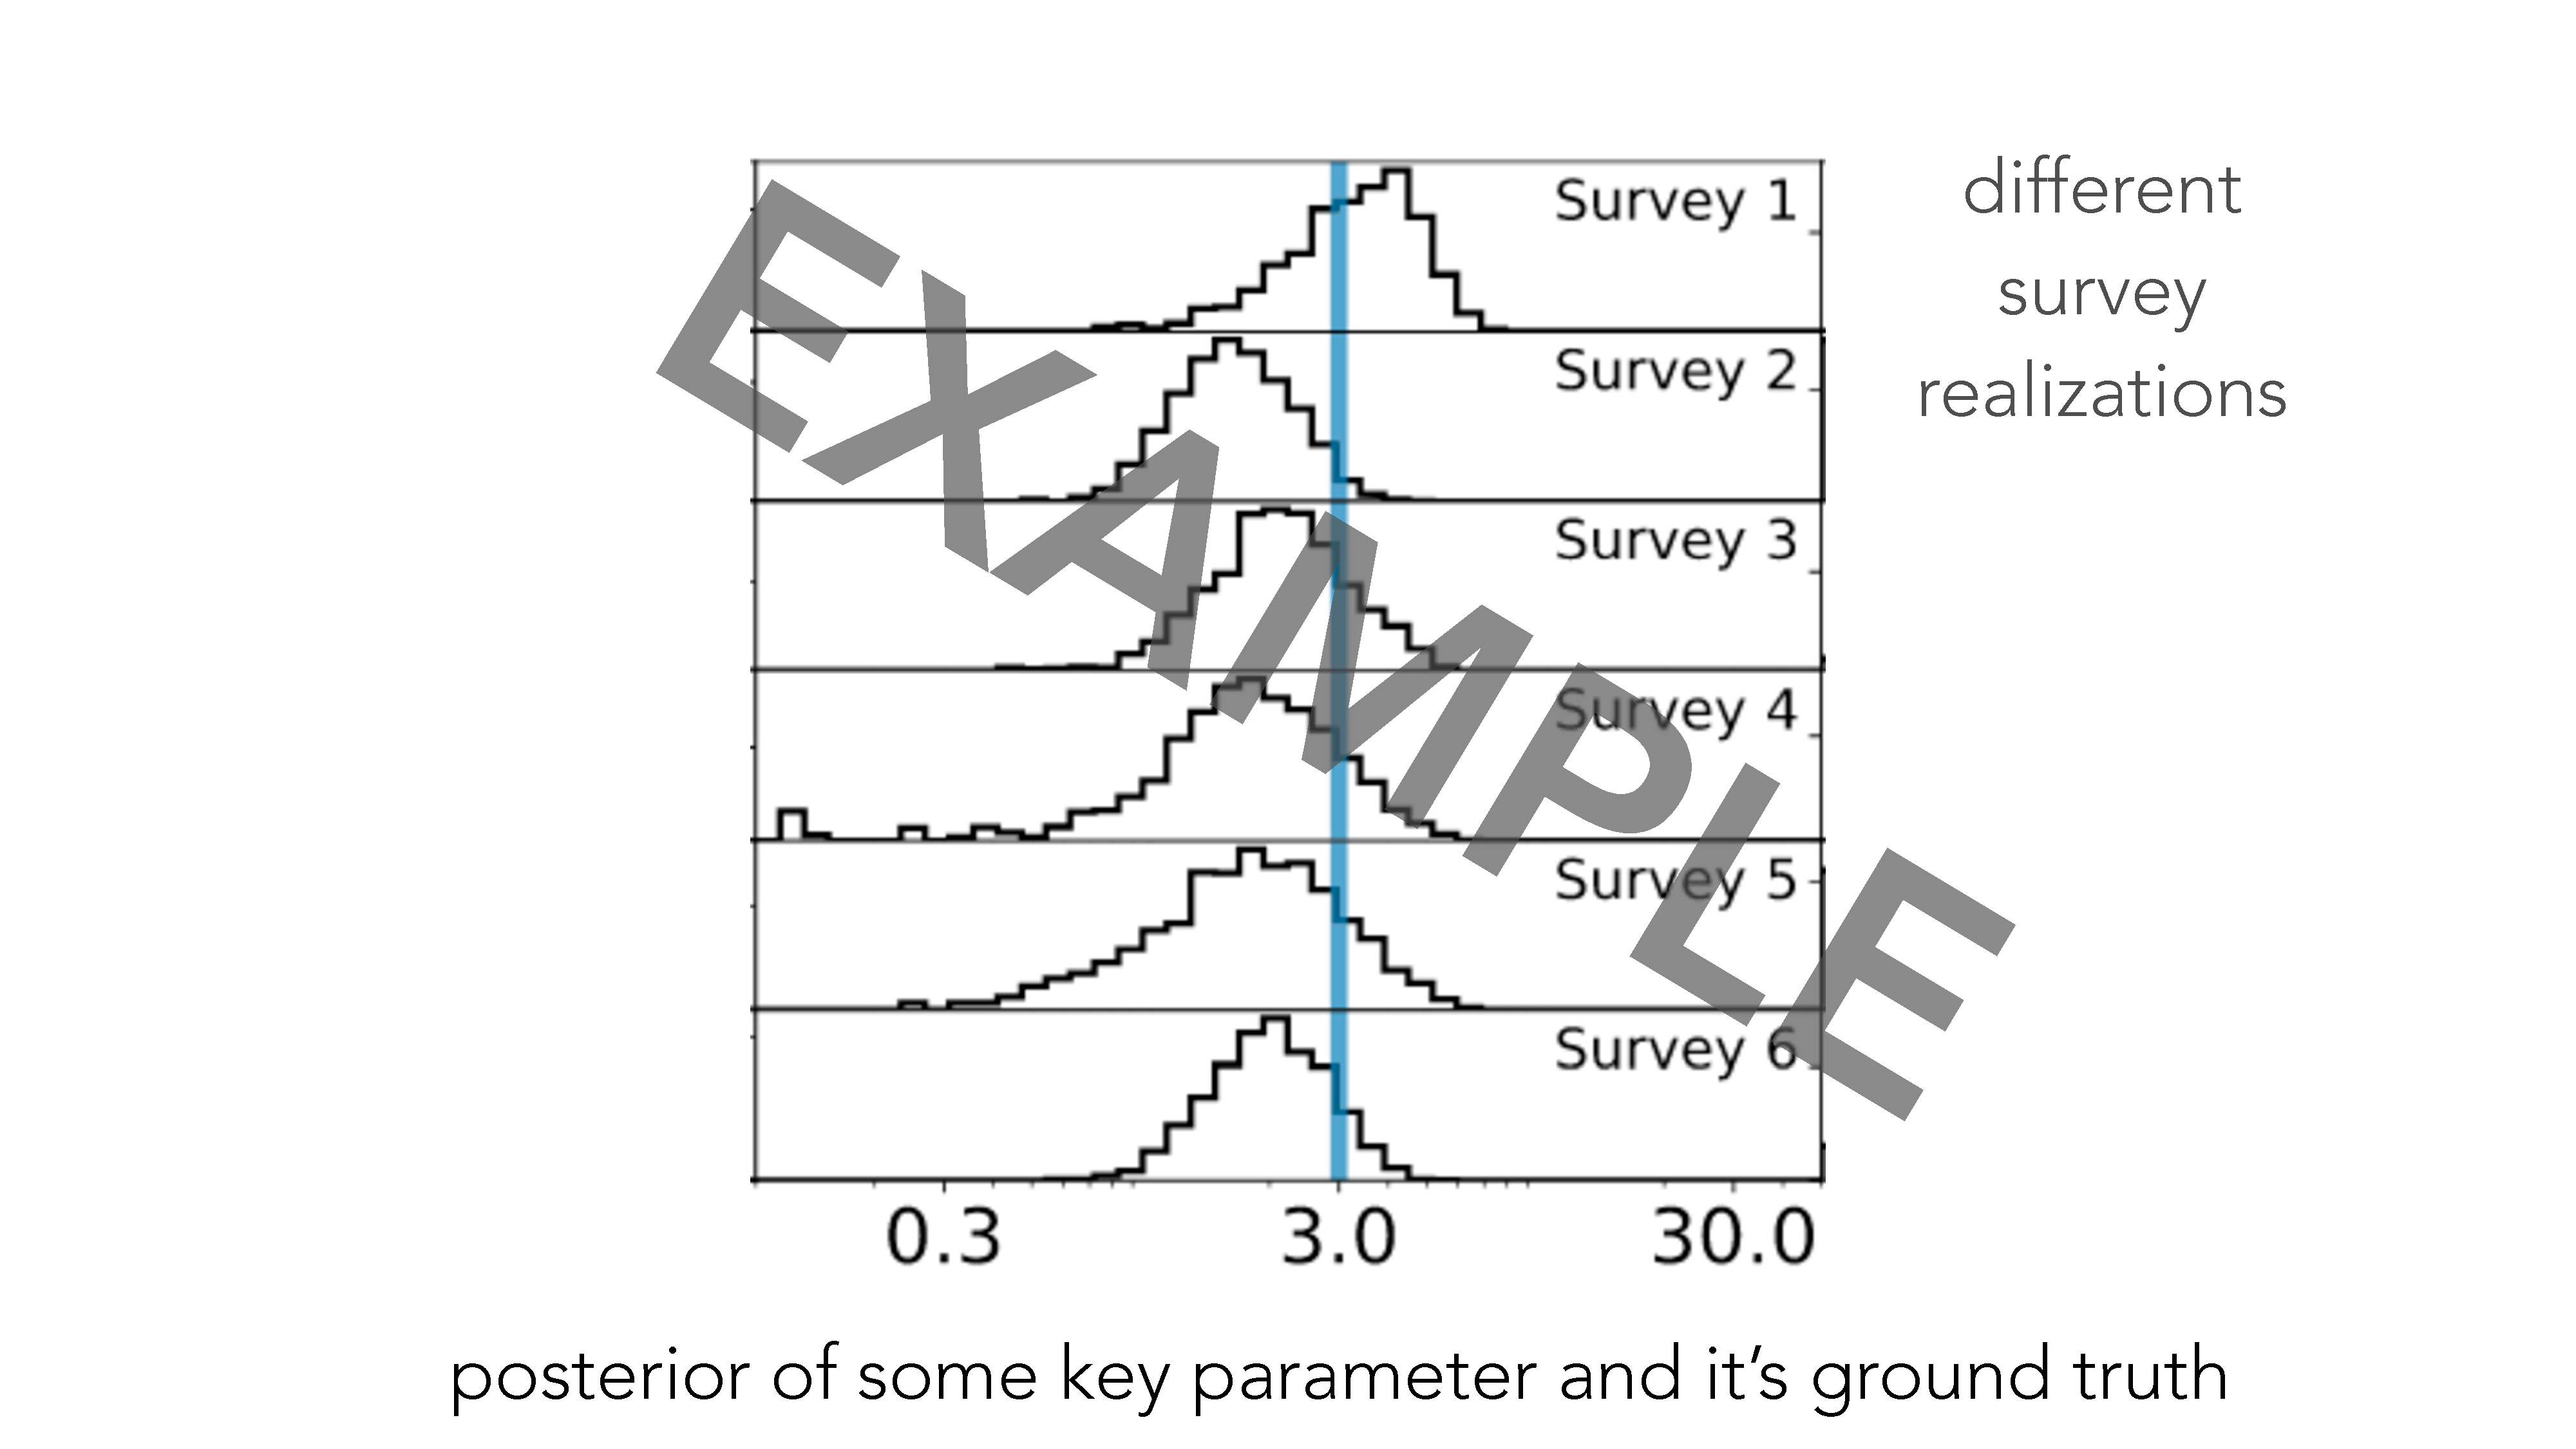
\includegraphics[width=\linewidth]{figures/example_posterior_surveys.pdf}
        \caption{
        Retrieved posterior distribution of the $<key parameter>$ for different survey realizations.
        The orange line corresponds to the true value of the injected signal.
        }
        \label{fig:posterior_surveys}
    \end{centering}
\end{figure}



\section{Conclusions}

\begin{note}
    \textit{Here or in the introduction:} For observations of rocky exoplanets, the currently best-probed regime that of hot, close-in planets.
    These bodies experience climatic conditions that are similar to the environment of the inner Solar System bodies at early stages of their formation.
    Studies of the geophysical state and evolution of hot exoplanets can thus contribute to our understanding of the early formation stages of Earth and other habitable worlds.
\end{note}


%\begin{acknowledgments}
%The authors thank Terry-Ann Suer for insightful discussions.
%\end{acknowledgements}

\begin{large}\textit{Author contributions:}\end{large}

\software{
Bioverse~\citep{Bixel2021},
Astropy~\citep[][]{AstropyCollaboration2018},
NumPy~\citep[][]{Harris2020},
SciPy~\citep[][]{Virtanen2020},
corner.py~\citep{Foreman-Mackey2016b}.
}


\bibliographystyle{aasjournal}
\bibliography{bib,PhD}
\end{document}